
\documentclass[tikz, border=10pt]{standalone}
\usepackage{tikz}
\usetikzlibrary{positioning, chains, shapes.geometric, fit, shapes, arrows.meta, calc, backgrounds}

\begin{document}
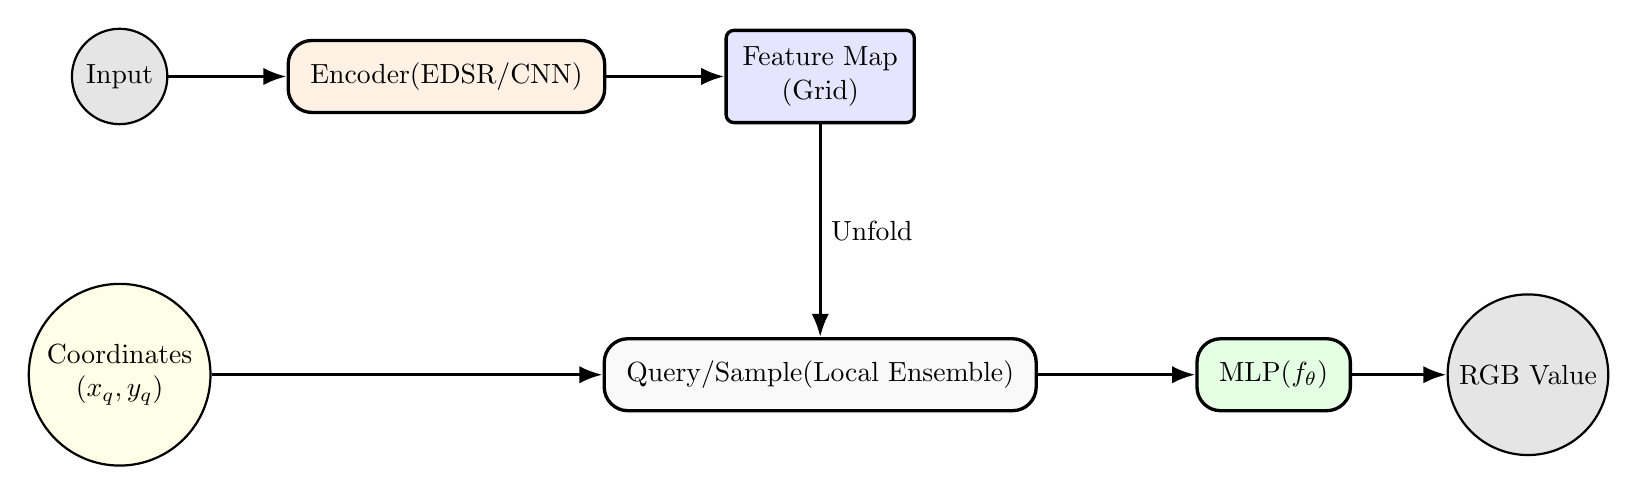
\begin{tikzpicture}[
    >=LaTeX, 
    very thick,
    node distance=1.0cm and 1.2cm,
    arrow/.style={
        ->,
        very thick,
        rounded corners=0.2cm
    },
    block/.style={
        rectangle,
        fill=gray!10,
        rounded corners=3mm,
        draw,
        very thick,
        inner sep=0.8em
    },
    layer/.style={
        rectangle,
        fill=white!10,
        rounded corners=1mm,
        inner xsep=0.6em,
        inner ysep=0.6em,
        minimum height=3.0em,
        align=center,
        draw,
        very thick
    },
    conv/.style={
        layer,
        fill=orange!10,
        draw=orange!80!black
    },
    relu/.style={
        layer,
        fill=yellow!10,
        draw=yellow!80!black,
        minimum height=2.5em
    },
    pool/.style={
        layer,
        fill=red!10,
        draw=red!80!black
    },
    input/.style={ 
        circle,
        minimum width=3.0em,
        draw,
        fill=gray!20,
        thick,
        align=center
    },
    sum/.style={
        circle,
        draw,
        fill=white,
        inner sep=0pt,
        minimum size=1.2em,
        node contents={+}
    }
]


    \node[input] (in) {Input};
    
    % Encoder
    \node[block, right=1.5cm of in, fill=orange!10] (encoder) {Encoder\\(EDSR/CNN)};
    \draw[arrow] (in) -- (encoder);

    % Feature Grid
    \node[layer, right=1.5cm of encoder, fill=blue!10] (feat) {Feature Map\\(Grid)};
    \draw[arrow] (encoder) -- (feat);

    % Coord Input
    \node[input, below=2.0cm of in, fill=yellow!10] (coord) {Coordinates\\$(x_q, y_q)$};
    
    % Sampling (Query)
    \node[block, at={(feat |- coord)}, fill=gray!5] (sample) {Query/Sample\\(Local Ensemble)};
    \draw[arrow] (coord) -- (sample);
    
    % Feature to Sample
    \draw[arrow] (feat.south) -- node[right]{Unfold} (sample.north);

    % MLP
    \node[block, right=2.0cm of sample, fill=green!10] (mlp) {MLP\\($f_\theta$)};
    \draw[arrow] (sample) -- (mlp);

    % Output
    \node[input, right=of mlp] (out) {RGB Value};
    \draw[arrow] (mlp) -- (out);

\end{tikzpicture}
\end{document}
